% Diploma-defense deck (Beamer) — ICS Anomaly Detection for Cyber-Physical Security
% Mirrors presentation/ICS_Anomaly_Detection_Defense.pptx. 18 frames, ~15 minutes.
% Build:  pdflatex -interaction=nonstopmode defense_slides.tex  (run twice for TikZ overlays)
\documentclass[aspectratio=169,11pt]{beamer}

\usepackage[utf8]{inputenc}
\usepackage[T1]{fontenc}
\usepackage{lmodern}
\usepackage{textcomp}
\usepackage{amssymb}
\usepackage{booktabs}
\usepackage{colortbl}
\usepackage{fancyvrb}
\usepackage{tikz}
\usetikzlibrary{positioning,arrows.meta,shapes.geometric}

\setbeamertemplate{navigation symbols}{}
\setbeamertemplate{itemize items}[circle]

% ---- palette -----------------------------------------------------------
\definecolor{navy}{RGB}{15,42,74}
\definecolor{teal}{RGB}{18,154,142}
\definecolor{ink}{RGB}{34,42,51}
\definecolor{muted}{RGB}{91,102,112}
\definecolor{lightbg}{RGB}{242,245,248}
\definecolor{rowalt}{RGB}{232,239,244}
\definecolor{kicker}{RGB}{191,228,224}

\setbeamercolor{normal text}{fg=ink}
\setbeamercolor{structure}{fg=teal}
\setbeamercolor{frametitle}{bg=navy,fg=white}
\setbeamercolor{itemize item}{fg=teal}
\setbeamercolor{itemize subitem}{fg=muted}
\setbeamerfont{frametitle}{size=\large,series=\bfseries}
\setbeamersize{text margin left=10mm,text margin right=8mm}

% frame title band with a teal rule + optional kicker (framesubtitle)
\setbeamertemplate{frametitle}{%
  \nointerlineskip%
  \begin{beamercolorbox}[wd=\paperwidth,sep=0pt,leftskip=8mm,rightskip=8mm]{frametitle}%
    \vskip2.2ex%
    {\usebeamerfont{frametitle}\insertframetitle}%
    \ifx\insertframesubtitle\@empty\else%
      \\[0.1ex]{\usebeamerfont*{framesubtitle}\color{kicker}\itshape\small\insertframesubtitle}%
    \fi%
    \vskip1.4ex%
  \end{beamercolorbox}%
  {\color{teal}\rule{\paperwidth}{1.2pt}}%
}

% footer
\setbeamertemplate{footline}{%
  \begin{beamercolorbox}[wd=\paperwidth,leftskip=8mm,rightskip=8mm,sep=0pt]{}%
  {\color{muted}\scriptsize ICS Anomaly Detection for Cyber-Physical Security\;\textperiodcentered\; IITU 2026\;\textperiodcentered\; \insertframenumber/18}\par\vspace{1.5mm}%
  \end{beamercolorbox}%
}

\newcommand{\arr}{\ensuremath{\rightarrow}}
\newcommand{\fig}[1]{../results/figures/#1}
\fvset{fontsize=\scriptsize,frame=single,framesep=3pt,rulecolor=\color{black!25},formatcom=\color{ink}}

% full-bleed navy frame helper text nodes via tikz
\newcommand{\bleed}{\begin{tikzpicture}[remember picture,overlay]\fill[navy](current page.south west)rectangle(current page.north east);\fill[teal](current page.west)++(0,0.0)rectangle++(\paperwidth,0.06);\end{tikzpicture}}

\begin{document}

% ===================================================================== 1 TITLE
{\setbeamertemplate{footline}{}
\begin{frame}[plain]
\begin{tikzpicture}[remember picture,overlay]
  \fill[navy](current page.south west)rectangle(current page.north east);
  \fill[teal]([yshift=10mm]current page.center-|current page.west)rectangle([yshift=9.0mm]current page.center-|current page.east);
  \node[anchor=north west,text width=0.9\paperwidth,align=left]
     at ([xshift=8mm,yshift=-6mm]current page.north west)
     {\color{kicker}\small International Information Technology University \textperiodcentered\ Faculty of Computer Technology and Cybersecurity};
  \node[anchor=west,text width=0.9\paperwidth,align=left]
     at ([xshift=8mm,yshift=22mm]current page.center-|current page.west)
     {\color{white}\bfseries\fontsize{30}{34}\selectfont ICS Anomaly Detection\\ for Cyber-Physical Security};
  \node[anchor=west,text width=0.9\paperwidth,align=left]
     at ([xshift=8mm,yshift=4mm]current page.center-|current page.west)
     {\color{teal}\bfseries\large Diploma Project \textperiodcentered\ Educational Program 6B06303 --- Network Security};
  \node[anchor=north west,text width=0.9\paperwidth,align=left]
     at ([xshift=8mm,yshift=-10mm]current page.center-|current page.west)
     {\color{white}\large\textbf{Team lead:\ Zainiddin Danial}\\[2pt]
      \color{white}\large Imankozhayeva Laura\\[2pt]
      \color{white}\large Bekisheva Galiya\\[6pt]
      \color{white}\normalsize Research advisor:\ Nurlybayev T.\,A.};
  \node[anchor=south west] at ([xshift=8mm,yshift=6mm]current page.south west)
     {\color{kicker}\normalsize Almaty 2026};
\end{tikzpicture}
\end{frame}}

% ===================================================================== 2 TEAM
\begin{frame}{Team composition \& roles}{Three students, three contributions of the thesis}
\small
\renewcommand{\arraystretch}{1.35}
\begin{tabular}{>{\raggedright\arraybackslash}p{2.6cm} >{\raggedright\arraybackslash}p{2.4cm} >{\raggedright\arraybackslash}p{7.6cm}}
\rowcolor{navy}\textcolor{white}{\textbf{Member}} & \textcolor{white}{\textbf{Role}} & \textcolor{white}{\textbf{Owns}}\\
\rowcolor{rowalt}\textbf{Zainiddin Danial} \textit{(lead)} & ML Engineering & Unified \texttt{AnomalyDetector} interface; the six detectors; experiment infrastructure \& reproducibility (YAML configs, config hash)\\
\textbf{Imankozhayeva Laura} & Data \& Evaluation & Data loaders \& preprocessing (scaler-leak guard); three time-aware metrics; cross-testbed transfer + within-HAI LOPO study\\
\rowcolor{rowalt}\textbf{Bekisheva Galiya} & Attribution \& Delivery & Per-sensor attribution + SHAP; inference/scoring pipeline; thesis writing and figures\\
\textbf{Nurlybayev T.\,A.} & Research advisor & Scope, methodology review, defense readiness\\
\end{tabular}
\end{frame}

% ===================================================================== 3 MOTIVATION
\begin{frame}{Why this matters: attacks on physical plants}{Industrial Control Systems run water, power, gas, chemicals}
\begin{center}
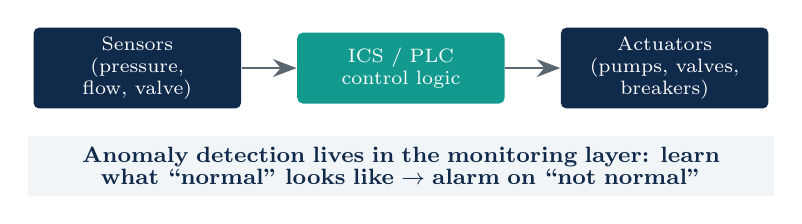
\begin{tikzpicture}[node distance=7mm,font=\scriptsize,
  box/.style={rectangle,rounded corners=2pt,minimum height=9mm,text width=24mm,align=center,text=white},
  arr/.style={-{Stealth[length=3mm]},muted,line width=1pt}]
  \node[box,fill=navy](a){Sensors\\(pressure, flow, valve)};
  \node[box,fill=teal,right=of a](b){ICS / PLC\\control logic};
  \node[box,fill=navy,right=of b](c){Actuators\\(pumps, valves, breakers)};
  \draw[arr](a)--(b); \draw[arr](b)--(c);
  \node[rectangle,fill=lightbg,text width=92mm,align=center,below=4mm of b,inner sep=4pt]
    {\color{navy}\bfseries\footnotesize Anomaly detection lives in the monitoring layer: learn what ``normal'' looks like \arr\ alarm on ``not normal''};
\end{tikzpicture}
\end{center}
\vspace{0.5mm}
\begin{itemize}\small\itemsep2pt
  \item \textbf{Stuxnet (2010)} --- malware physically destroyed centrifuges while screens showed normal readings
  \item \textbf{Ukraine power grid (2015)} --- attackers tripped breakers, $\sim$225,000 customers blacked out in winter
  \item \textbf{Maroochy Shire (2000)} --- stolen radio opened sewage valves, $\sim$1 million litres spilled
  \item[\color{teal}\checkmark] \textbf{In every case the attack was visible in the sensor data --- if someone watched the right pattern.}
\end{itemize}
\end{frame}

% ===================================================================== 4 TASK
\begin{frame}{Task statement}{What the diploma sets out to prove and build}
\begin{block}{}
{\color{teal}\bfseries Thesis:} ICS detectors report high F1 on their training dataset, but (a) their rankings change under time-aware metrics and (b) they fail to generalize across testbeds. We quantify both effects on HAI and Morris, and add per-sensor attribution to evaluate detection \emph{and} localization.
\end{block}
\begin{enumerate}\small\itemsep2pt
  \item Survey ICS anomaly-detection methods, datasets, and time-aware evaluation metrics
  \item Implement six detectors under one \texttt{AnomalyDetector} interface (fit / score / attribute)
  \item Implement three metrics with unit tests; reproduce published baselines within tolerance
  \item Cross-testbed transfer HAI $\leftrightarrow$ Morris (source- vs target-calibrated) + within-HAI leave-one-process-out
  \item Per-sensor attribution vs HAI process-level attack labels, with multi-seed sensitivity
  \item Findings, practical recommendations, and a reproducible apparatus
\end{enumerate}
\end{frame}

% ===================================================================== 5 DATASETS
\begin{frame}{The two testbeds}{Deliberately dissimilar --- that is the point}
\begin{columns}[T]
\begin{column}{0.52\textwidth}
\scriptsize
\renewcommand{\arraystretch}{1.25}
\begin{tabular}{>{\raggedright\arraybackslash}p{1.7cm} >{\raggedright\arraybackslash}p{2.6cm} >{\raggedright\arraybackslash}p{2.6cm}}
\rowcolor{navy}\textcolor{white}{\textbf{}} & \textcolor{white}{\textbf{HAI 21.03}} & \textcolor{white}{\textbf{Morris}}\\
\rowcolor{rowalt}\textbf{Domain} & Power-plant (boiler, turbine, water) & Gas-pipeline Modbus RTU\\
\textbf{Features} & 79 sensor channels & 16 features\\
\rowcolor{rowalt}\textbf{Processes} & 4 interconnected (P1--P4) & Single pipeline\\
\textbf{Rate} & 1\,Hz, timestamped & Sub-second, none\\
\rowcolor{rowalt}\textbf{Format} & Folder of CSVs & ARFF file\\
\textbf{Shared} & \multicolumn{2}{c}{--- no sensors in common ---}\\
\end{tabular}
\end{column}
\begin{column}{0.46\textwidth}
\centering

\includegraphics[height=0.55\textheight]{\fig{01_exploration/hai_overview.png}}\\[1mm]
{\color{muted}\scriptsize HAI: 79 channels across four physical loops}
\end{column}
\end{columns}
\end{frame}

% ===================================================================== 6 MODELS
\begin{frame}{Six detectors, one interface}{Two classical \textperiodcentered\ two autoencoders \textperiodcentered\ two transformer-era SOTA}
\renewcommand{\arraystretch}{1.3}\small
\begin{tabular}{>{\raggedright\arraybackslash}p{3.2cm} >{\raggedright\arraybackslash}p{2.2cm} p{1.2cm} >{\raggedright\arraybackslash}p{6.0cm}}
\rowcolor{navy}\textcolor{white}{\textbf{Model}} & \textcolor{white}{\textbf{Family}} & \textcolor{white}{\textbf{Year}} & \textcolor{white}{\textbf{Core idea}}\\
\rowcolor{rowalt}Isolation Forest & Classical & 2008 & Random splits isolate outliers faster\\
One-Class SVM & Classical & 2001 & Boundary around the normal region\\
\rowcolor{rowalt}Dense Autoencoder & Autoencoder & --- & High reconstruction error = anomaly\\
LSTM Autoencoder & Autoencoder & 2016 & Sequence reconstruction over time\\
\rowcolor{rowalt}USAD & SOTA & 2020 & Adversarially-trained autoencoder pair\\
TranAD & SOTA & 2022 & Transformer: attention + adversarial loss\\
\end{tabular}
\vspace{2mm}
\begin{center}\small\color{muted}Swapping any model is a one-line config change --- apples-to-apples by construction.\end{center}
\end{frame}

% ===================================================================== 7 METRICS
\begin{frame}{Three time-aware metrics}{How you score a detector changes who wins}
\begin{columns}[T]
\foreach \tt/\bd/\nt/\cl in {%
  {Point-wise F1}/{Standard per-timestep precision / recall / F1.}/{Honest but unforgiving on short events.}/{navy},
  {Point-adjust F1}/{Flag \emph{any} point in an attack and the whole attack counts as detected.}/{Inflated --- a random flagger beats real detectors (Kim et al., AAAI 2022).}/{red!55!black},
  {eTaPR}/{Event-aware: rewards how much of each attack you catch and how fast.}/{The honest metric we trust for ranking.}/{teal}}{%
\begin{column}{0.32\textwidth}
  \begin{beamercolorbox}[wd=\textwidth,ht=3.2ex,center]{}\colorbox{\cl}{\makebox[\textwidth][c]{\color{white}\bfseries\strut \tt}}\end{beamercolorbox}
  \vspace{2mm}{\small \bd}\\[3mm]{\small\color{\cl}\itshape\bfseries \nt}
\end{column}}
\end{columns}
\vspace{4mm}
\begin{center}\small\color{muted}We report all three --- because the ranking changes between them, and that change is a finding.\end{center}
\end{frame}

% ===================================================================== 8 ARCHITECTURE
\begin{frame}{System architecture}{Config-driven, reproducible, no hidden state}
\begin{center}
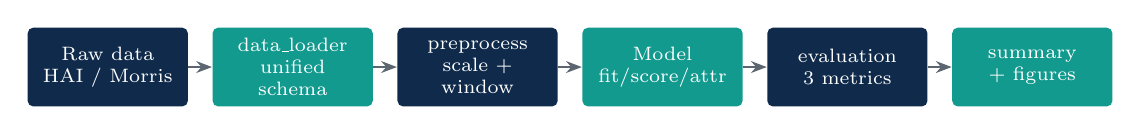
\begin{tikzpicture}[font=\scriptsize,node distance=3.0mm,
  b/.style={rectangle,rounded corners=2pt,minimum height=10mm,text width=18mm,align=center,text=white},
  ar/.style={-{Stealth[length=2mm]},muted,line width=0.8pt}]
  \node[b,fill=navy](a){Raw data\\HAI / Morris};
  \node[b,fill=teal,right=of a](b){data\_loader\\unified schema};
  \node[b,fill=navy,right=of b](c){preprocess\\scale + window};
  \node[b,fill=teal,right=of c](d){Model\\fit/score/attr};
  \node[b,fill=navy,right=of d](e){evaluation\\3 metrics};
  \node[b,fill=teal,right=of e](f){summary\\+ figures};
  \draw[ar](a)--(b);\draw[ar](b)--(c);\draw[ar](c)--(d);\draw[ar](d)--(e);\draw[ar](e)--(f);
\end{tikzpicture}
\end{center}
\vspace{1mm}
\begin{itemize}\itemsep3pt
  \item One \texttt{AnomalyDetector} base class --- \texttt{fit / score / attribute / save / load} --- every model obeys it
  \item Every experiment is a YAML config; the runner is model-agnostic
  \item Each run records a 12-char config hash + seed + timestamp \arr\ one row in \texttt{summary.parquet}
  \item Notebooks only plot. If a number is in the thesis, a tested function in \texttt{src/} produced it
\end{itemize}
\end{frame}

% ===================================================================== 9 TRANSFER METHOD
\begin{frame}{Bridging two testbeds: the type vector}{If they share no sensors, compare sensor \textsc{types}}
\begin{center}
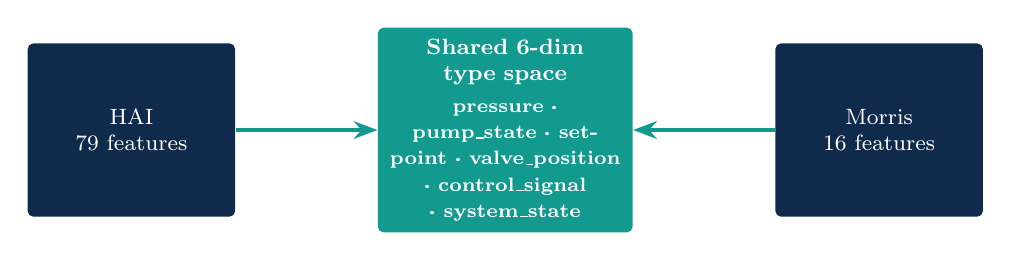
\begin{tikzpicture}[font=\footnotesize,
  big/.style={rectangle,rounded corners=2pt,minimum height=22mm,text width=24mm,align=center,text=white},
  ar/.style={-{Stealth[length=3mm]},teal,line width=1.2pt}]
  \node[big,fill=navy](h){HAI\\79 features};
  \node[rectangle,rounded corners=2pt,fill=teal,text=white,text width=30mm,align=center,minimum height=26mm,right=18mm of h](m)
     {\bfseries Shared 6-dim\\ type space\\[2pt]\scriptsize pressure \textperiodcentered\ pump\_state \textperiodcentered\ setpoint \textperiodcentered\ valve\_position \textperiodcentered\ control\_signal \textperiodcentered\ system\_state};
  \node[big,fill=navy,right=18mm of m](mo){Morris\\16 features};
  \draw[ar](h)--(m);\draw[ar](mo)--(m);
\end{tikzpicture}
\end{center}
\begin{itemize}\itemsep2pt\small
  \item Each sensor hand-tagged by \textsc{type} in \texttt{data/feature\_types.yaml} (pressure, valve, control signal\ldots)
  \item Both datasets projected onto the shared 6-dim type vector \arr\ models become transferable
  \item Transfer the \emph{scoring function}, not the raw weights --- methodologically the cleanest option
\end{itemize}
\end{frame}

% ===================================================================== 10 SOFTWARE
\begin{frame}{Software \& reproducibility}{Tooling and the build-everything-from-config rule}
\begin{itemize}\itemsep4pt
  \item[\color{teal}\textbf{1.}] \textbf{Languages \& ML:}\ Python 3.11 \textperiodcentered\ PyTorch 2.3 \textperiodcentered\ scikit-learn 1.4 \textperiodcentered\ NumPy / pandas
  \item[\color{teal}\textbf{2.}] \textbf{Explainability \& artifacts:}\ SHAP (classical attribution) \textperiodcentered\ joblib model artifacts \textperiodcentered\ CLI scoring of fresh data
  \item[\color{teal}\textbf{3.}] \textbf{Quality \& docs:}\ pytest 8.0 (13 test modules) \textperiodcentered\ ruff \textperiodcentered\ pre-commit \textperiodcentered\ LaTeX (thesis + figures)
  \item[\color{teal}\textbf{4.}] \textbf{Reproducibility contract:}\ \texttt{python -m experiments.run <config.yaml>} \arr\ one row in \texttt{results/metrics/summary.parquet}
  \item[] \hspace{6mm}$\sim$48 YAML configs \textperiodcentered\ 12-char config hash \textperiodcentered\ seeds 7 / 42 / 123 \textperiodcentered\ Parquet for nested metrics
\end{itemize}
\end{frame}

% ===================================================================== 11 IMPLEMENTATION
\begin{frame}[fragile]{Implementation --- key points}{The interface contract and the anti-leakage guard}
\begin{columns}[T]
\begin{column}{0.5\textwidth}
{\color{navy}\bfseries\footnotesize src/models/base.py --- every model obeys this}
\begin{Verbatim}
class AnomalyDetector(ABC):
    @abstractmethod
    def fit(self, X_train, X_val=None):
        # Fit on normal-only data.
        # Must never see attack rows.
        ...
    @abstractmethod
    def score(self, X):
        # per-sample anomaly score
        ...
    def attribute(self, X):
        # per-feature contribution
        ...
\end{Verbatim}
\end{column}
\begin{column}{0.5\textwidth}
{\color{navy}\bfseries\footnotesize src/preprocessing.py --- scaler-leak guard}
\begin{Verbatim}
def scale_bundle(bundle):
    # #1 cause of inflated ICS results:
    # fitting the scaler on attack rows.
    # Crash rather than trust callers.
    bundle.assert_no_attack_in_train_val()

    scaler = MinMaxScaler(clip=True)
    scaler.fit(X_train)   # normal only
    return ScaledArrays(...)
\end{Verbatim}
\vspace{0.5mm}
\begin{block}{Deployable model artifact}
\scriptsize Model + scaler + threshold + metadata save as one unit; scoring fresh data is one call --- \texttt{score\_dataframe(artifact, df)}.
\end{block}
\end{column}
\end{columns}
\end{frame}

% ===================================================================== 12 DETECTION
\begin{frame}{Results --- same-dataset detection}{Point-wise F1 / ROC-AUC, scaler fit on normal only}
\begin{columns}[T]
\begin{column}{0.48\textwidth}
\renewcommand{\arraystretch}{1.3}\small
\begin{tabular}{>{\raggedright\arraybackslash}p{2.6cm} c c c c}
\rowcolor{navy}\textcolor{white}{\textbf{Model}} & \textcolor{white}{\textbf{H-F1}} & \textcolor{white}{\textbf{H-AUC}} & \textcolor{white}{\textbf{M-F1}} & \textcolor{white}{\textbf{M-AUC}}\\
\rowcolor{rowalt}Dense AE & 0.524 & 0.859 & 0.737 & 0.751\\
Isolation Forest & 0.208 & 0.770 & 0.734 & 0.658\\
\rowcolor{rowalt}One-Class SVM & 0.307 & 0.757 & 0.653 & 0.629\\
LSTM AE & 0.148 & 0.670 & 0.9997 & ---\\
\end{tabular}
\vspace{3mm}
\begin{itemize}\scriptsize\itemsep2pt
  \item Dense AE leads on HAI; absolute F1 modest (0.52) even at home
  \item High Morris F1 partly reflects its $\sim$91\% windowed attack rate --- a warning sign
\end{itemize}
\end{column}
\begin{column}{0.50\textwidth}
\centering

\includegraphics[height=0.72\textheight]{\fig{04_sota/sota_six_model_comparison.png}}
\end{column}
\end{columns}
\end{frame}

% ===================================================================== 13 METRIC SENSITIVITY
\begin{frame}{Results --- metric sensitivity}{The same models, re-ranked by the metric}
\begin{columns}[c]
\begin{column}{0.66\textwidth}
\centering
\includegraphics[width=\textwidth]{\fig{06_metric_sensitivity/metric_sensitivity.png}}
\end{column}
\begin{column}{0.32\textwidth}
\begin{itemize}\itemsep5pt
  \item \textbf{Rankings shuffle} between point-wise, PA-F1, eTaPR
  \item \textbf{PA-F1 inflates} classical detectors most
  \item \textbf{Takeaway:} a single-metric leaderboard is unreliable
\end{itemize}
\end{column}
\end{columns}
\end{frame}

% ===================================================================== 14 TRANSFER RESULTS
\begin{frame}{Results --- cross-testbed transfer\ \ (headline)}{Calibration, not the model, decides whether transfer means anything}
\begin{columns}[c]
\begin{column}{0.5\textwidth}\centering
\includegraphics[height=0.48\textheight]{\fig{05_cross_dataset/transfer_calibration_comparison.png}}\end{column}
\begin{column}{0.5\textwidth}\centering
\includegraphics[height=0.48\textheight]{\fig{05_cross_dataset/lopo_heatmap.png}}\end{column}
\end{columns}
\vspace{0.5mm}
\begin{itemize}\scriptsize\itemsep1pt
  \item \textbf{Source-calibrated transfer collapses every detector to the target's class-prior baseline} (F1 $\approx$ 0.95 Morris, $\approx$ 0.05 HAI) --- the number reflects base rates, not intelligence.
  \item Target-calibrating on normal target data restores meaning: SOTA reaches 0.38--0.44 eTaPR (HAI\arr Morris); classical stays below 0.13.
  \item Within-HAI LOPO (right): hiding a process's sensors causes \emph{targeted} blindness, not uniform decay.
\end{itemize}
\end{frame}

% ===================================================================== 15 ATTRIBUTION
\begin{frame}{Results --- attribution \& localization}{``We caught it'' $\neq$ ``here's which sensor''}
\begin{columns}[c]
\begin{column}{0.5\textwidth}\centering
\includegraphics[height=0.49\textheight]{\fig{07_attribution/attribution_p_at_5.png}}\end{column}
\begin{column}{0.5\textwidth}\centering
\includegraphics[height=0.49\textheight]{\fig{07_attribution/shap_if_ocsvm_pak.png}}\end{column}
\end{columns}
\vspace{0.5mm}
\begin{itemize}\scriptsize\itemsep1pt
  \item \textbf{Detection-vs-localization inversion:} the Dense AE --- weakest by F1 --- is the only windowed/AE model above random on all three attacked HAI processes.
  \item Attention rollout (TranAD) is numerically identical to reconstruction error --- a null result.
  \item SHAP lifts the two classical baselines above random too (right).
\end{itemize}
\end{frame}

% ===================================================================== 16 FINDINGS
\begin{frame}{Key findings \& recommendations}{Three findings $\rightarrow$ three things a security team should do}
\begin{columns}[T]
\begin{column}{0.49\textwidth}
{\color{teal}\bfseries\large Findings}
\begin{enumerate}\small\itemsep6pt
  \item Naive cross-factory transfer collapses to coin-flipping (class-prior baseline).
  \item Hiding one subsystem's sensors causes \emph{targeted} blindness, not global decay.
  \item The worst detector (Dense AE) is the best localizer; attention explanations are null.
\end{enumerate}
\end{column}
\begin{column}{0.49\textwidth}
\begin{block}{\color{navy}Recommendations}
\small
\begin{itemize}\itemsep5pt
  \item[\color{teal}\checkmark] Calibrate the threshold on \emph{target}-domain normal data before deploying a transferred detector.
  \item[\color{teal}\checkmark] Report multiple time-aware metrics (incl.\ eTaPR); distrust single-metric rankings.
  \item[\color{teal}\checkmark] Audit attribution alongside detection --- consider a SOTA-detector + Dense-AE/SHAP-localizer hybrid.
\end{itemize}
\end{block}
\end{column}
\end{columns}
\end{frame}

% ===================================================================== 17 CONCLUSION
\begin{frame}{Conclusion}{A measurement project, shipped reproducibly}
\begin{itemize}\itemsep4pt
  \item Benchmarked six detectors on HAI and Morris under three time-aware metrics
  \item Separated representation transfer from threshold transfer --- exposing how published F1 misleads
  \item Established a detection-vs-localization tradeoff via per-sensor attribution
\end{itemize}
\vspace{1mm}
{\color{teal}\bfseries Contributions:}
\begin{itemize}\itemsep3pt
  \item A reproducible benchmarking protocol --- every number rebuilds from a committed YAML
  \item An open-source implementation under one detector interface (7th model = one class)
  \item A recommendation to the field: report the \emph{full grid} --- metrics $\times$ calibration $\times$ attribution --- not a single headline F1
\end{itemize}
\end{frame}

% ===================================================================== 18 THANKS
{\setbeamertemplate{footline}{}
\begin{frame}[plain]
\begin{tikzpicture}[remember picture,overlay]
  \fill[navy](current page.south west)rectangle(current page.north east);
  \fill[teal]([yshift=4mm]current page.center-|current page.west)rectangle([yshift=3.0mm]current page.center-|current page.east);
  \node at ([yshift=20mm]current page.center){\color{white}\bfseries\fontsize{30}{34}\selectfont Thank you for your attention};
  \node at ([yshift=-8mm]current page.center){\color{teal}\large\bfseries ICS Anomaly Detection for Cyber-Physical Security};
  \node at ([yshift=-18mm]current page.center){\color{white}\normalsize Zainiddin Danial \textperiodcentered\ Imankozhayeva Laura \textperiodcentered\ Bekisheva Galiya};
  \node at ([yshift=-26mm]current page.center){\color{kicker}\small Advisor: Nurlybayev T.\,A. \textperiodcentered\ IITU, Almaty 2026};
\end{tikzpicture}
\end{frame}}

\end{document}
